\documentclass[main.tex]{subfiles}
\ifxetex\else\onlyinsubfile{\usepackage{CJKutf8}}\fi
\begin{document}
\ifxetex\else\begin{CJK*}{UTF8}{song}\fi

\chapter{SD卡和文件系统}
计算机的存储系统分为内存和外存。第四章讲了内存管理的一部分,本章来讲外存管理。因为树莓派的 SoC集成了 EMMC控制器,可以直接访问 (micro)SD卡,SD卡自然是最便捷的外存。如果安装了 rasp\-bian, SD卡上一般有两个分区,其中一个分区是 FAT文件系统,而另一个是 ext4文件系统。其中, FAT文件系统中包含了引导程序 (boot\-code.bin, start.elf)及其参数 (config.txt)和 Linux内核 kernel.img等文件,而 ext4分区保存了 rasp\-bian除内核外的其他文件。如果没有安装 rasbpian,一般只有一个FAT分区。

\par
关于文件系统的设计与实现,已经有很多资料。本章不会深入去讲解如何访问 SD卡,也不会设计并实现一个新的文件系统,甚至不会讲解已有文件系统的设计与实现。我们只是以 SD卡上的 FAT文件系统为例子,着重关注接口设计与封装,以让我们的操作系统能够访问 SD卡上的 FAT文件系统。

\par
本章中关于 SD卡读写和 FAT文件系统的实现,均采用了开源代码,具体来源请参考文件 sd\-card.c和 dos\-fs.c中的说明。

\section{设备接口}
一般来说,文件系统存储在设备上。因此,先要对底层设备做一个抽象,然后在此基础上构建文件系统。对于设备来说,驱动接口主要包括连接、断开、读写、查询和 I/O控制等,如代码\ref{code:6-1}所示。

\begin{code}
\captionof{listing}{chapter06/kernel/kernel.h}
\label{code:6-1}
\inputminted[firstline=135,lastline=157,linenos,numbersep=5pt,frame=lines,framesep=2mm]{c}{src/chapter06/kernel/kernel.h}
\end{code}

\noindent
简单解释一下各个接口函数的功能。

\begin{itemize}
\item major是一个字符串,表示驱动的名称。
\item attach/detach用于连接/断开设备。
\item read从设备中读取数据,参数 addr指定了开始读取的地址。注意,有些设备上的数据没有地址,比如键盘、鼠标或网卡等。对于这种设备,可以忽略该参数。
\item write往设备中写入数据。
\item poll向设备查询输入输出状态。
\item ioctl是设备的 I/O控制接口,用于向设备发送控制命令。
\end{itemize}

有了驱动接口,接下来用 struct dev去描述设备。可以看出,结构体 dev只包含了驱动接口指针和设备号。驱动接口的指针指定了设备的类别,而设备号用于区分同一类设备的不同实例。具体来说,驱动接口中的 major字段给出了设备类别的名称,而设备中的 minor字段表示该类别的第几个设备。这种设计类似于 Unix/Linux中的主次设备号,但它们都是数字。显然,在实现具体的设备时,一般要对 struct dev进行扩充。用 C++的话来说,即具体的设备要从 dev继承。

\par
全局变量 g\_dev\_vector包含了系统支持的所有设备的列表。

\section{SD卡实现}
下面以 SD卡为例实现上面的驱动接口。

\begin{code}
\captionof{listing}{chapter06/kernel/sdcard.c}
\label{code:6-2}
\inputminted[firstline=1737,lastline=1754,linenos,numbersep=5pt,frame=lines,framesep=2mm]{c}{src/chapter06/kernel/sdcard.c}
\end{code}

首先,根据 SoC的 EMMC控制器操作手册,实现了接口函数 sd\_\-attach/\-detach/\-read/\-write/\-poll/\-ioctl。然后,定义一个描述 SD卡的结构体 sd\_dev,并填入驱动接口地址和设备号。 SD卡的读写细节比较繁杂,不是这里的重点,因此不在这里列出,请自行看源代码。

\section{文件系统接口}
接下来设计文件系统的接口,如代码\ref{code:6-3}所示。

\begin{code}
\captionof{listing}{chapter06/kernel/kernel.h}
\label{code:6-3}
\inputminted[firstline=159,lastline=189,linenos,numbersep=5pt,frame=lines,framesep=2mm]{c}{src/chapter06/kernel/kernel.h}
\end{code}

\noindent
这个接口类似于 Unix/Linux中的设计,各个函数的功能如下:

\begin{itemize}
\item mount用于挂载文件系统,参数dev和addr指定了文件系统位于哪个设备的哪个地址上。
\item unmount用于卸载文件系统。
\item open用于打开一个文件,path指定了路径,mode是打开模式。
\item close用于关闭文件。
\item read从文件中读取数据。
\item write往文件中写入数据。
\item seek用于移动读写指针,成功时返回新的读写指针。
\end{itemize}

\noindent
文件用 struct file描述,它只包含了文件系统接口的指针。将来具体实现某种文件系统时,要对它进行扩充,亦即从它继承。

\par
全局变量 g\_fs\_vector包含了系统支持的所有文件系统,而 g\_file\_vector记录了系统打开的所有文件。

\section{FAT文件系统实现}
下面以 FAT文件系统为例子,看看如何实现文件系统的接口。

\begin{code}
\captionof{listing}{chapter06/kernel/dosfs.c}
\label{code:6-4}
\inputminted[firstline=1337,lastline=1359,linenos,numbersep=5pt,frame=lines,framesep=2mm]{c}{src/chapter06/kernel/dosfs.c}
\end{code}

首先,定义一个 struct fat\_file来描述 FAT文件系统中的一个文件,里面除了 file字段之外,还有一个 FAT所特有的字段 FILEINFO。

\par
接下来是 struct fat\_fs,它描述了 FAT文件系统,除了 struct fs之外,还要记录该文件系统在哪个设备 dev上,以及 FAT特定的 VOLINFO字段。因为文件系统尚未挂载,所以 dev和 VOLINFO都填入 0。

\par
在第三方代码的基础上,接口函数的封装比较简单,不在这里列出,请自行看源代码。

\section{设备文件系统实现}
熟悉 Unix/Linux的读者知道,它们支持所谓的设备文件系统,即“/dev”文件系统。我们也可以做一个功能类似的设备文件系统,作为除FAT之外的另一个例子。

\begin{code}
\captionof{listing}{chapter06/kernel/devfs.c}
\label{code:6-5}
\inputminted[firstline=12,lastline=31,linenos,numbersep=5pt,frame=lines,framesep=2mm]{c}{src/chapter06/kernel/devfs.c}
\end{code}

\noindent
设备文件 struct dev\_\-file中除了 file之外,还有设备对象 dev,打开模式 mode和读写指针。

\par
在我们的操作系统中,对于系统中的每个设备,采用“driver.major + dev.minor”的命名方式,即如果驱动接口中的 major是“sd”,那么第一个设备的名称用 sd0表示,第二个 sd1,以此类推。

\par
下面先看一下 devfs\_\-open函数的实现。 52~ 60行,对于用户提供的文件名 name,在设备列表 g\_dev\_vector中查找,看是否有匹配的设备。如果有, 62行调用驱动接口中的 attach进行连接,连接成功后, 65~ 71行创建文件对象,并填充相关字段。

\begin{code}
\captionof{listing}{chapter06/kernel/devfs.c}
\label{code:6-6}
\inputminted[firstline=43,lastline=74,linenos,numbersep=5pt,frame=lines,framesep=2mm]{c}{src/chapter06/kernel/devfs.c}
\end{code}

\noindent
再来看一下devfs\_\-read的实现。它只是调用了驱动接口的 read函数,把数据从设备读到用户提供的内存中,然后移动读写指针。

\begin{code}
\captionof{listing}{chapter06/kernel/devfs.c}
\label{code:6-7}
\inputminted[firstline=83,lastline=98,linenos,numbersep=5pt,frame=lines,framesep=2mm]{c}{src/chapter06/kernel/devfs.c}
\end{code}

\noindent
其他的接口函数实现也比较简单,这里不再列出。

\section{用户接口}
在我们的操作系统中,文件系统采用类似于 Windows的命名方法,即一个文件系统用一个字母来表示,比如 A:表示第一个文件系统, B:表示第二个,以此类推。对于设备文件系统,用\$:表示。所以,“A:/a.out”表示第一个文件系统根目录下面的 a.out文件,而\$:/sd0表示第一个 SD卡。

\par
用户接口主要包括函数 sys\_open/\-close/\-read/\-write/\-seek。这里只列出 sys\_\-open的实现,如代码\ref{code:6-8}所示。

\begin{code}
\captionof{listing}{chapter06/kernel/file.c}
\label{code:6-8}
\inputminted[firstline=6,lastline=45,linenos,numbersep=5pt,frame=lines,framesep=2mm]{c}{src/chapter06/kernel/file.c}
\end{code}

\noindent
它根据用户提供的文件路径 path,在 g\_fs\_vector中找到对应的文件系统,然后调用它的 open即可。成功后,把文件对象保存在 g\_file\_vector中,然后返回它在这个向量中的索引作为文件描述符 (file descriptor, fd)。

\section{测试}
先初始化 SD卡,并挂载设备文件系统和 FAT文件系统。注意,设备文件系统是一个虚拟的文件系统,它不需要存储在设备上,而 FAT文件系统位于 SD卡上。

\begin{code}
\captionof{listing}{chapter06/kernel/machdep.c}
\label{code:6-9}
\inputminted[firstline=516,lastline=531,linenos,numbersep=5pt,frame=lines,framesep=2mm]{c}{src/chapter06/kernel/machdep.c}
\end{code}

接下来,可以测试文件的各个操作。首先,读取一个普通文件,即 A:/kernel.img。然后,通过设备文件\$:/sd0直接访问 SD卡的原始数据。特别注意,在通过设备文件修改 SD卡上的数据时,可能会破坏里面的文件系统!!

\begin{code}
\captionof{listing}{chapter06/kernel/machdep.c}
\label{code:6-10}
\inputminted[firstline=533,lastline=576,linenos,numbersep=5pt,frame=lines,framesep=2mm]{c}{src/chapter06/kernel/machdep.c}
\end{code}

为了保持屏幕整洁以便于观察,我们去掉了第三章定时器中断的输出,即“.”。测试结果如图\ref{figure:6-1}所示。你可以自己比较一下 kernel.img的内容,看看是否正确。事实上,测试设备文件\$:/sd0时,测试代码读取了 SD卡的主引导记录(Master Boot Record, MBR)中的分区表和结束标志“55 AA”。 MBR位于 SD卡的第一个扇区。

\begin{figure}[htp]
\centering
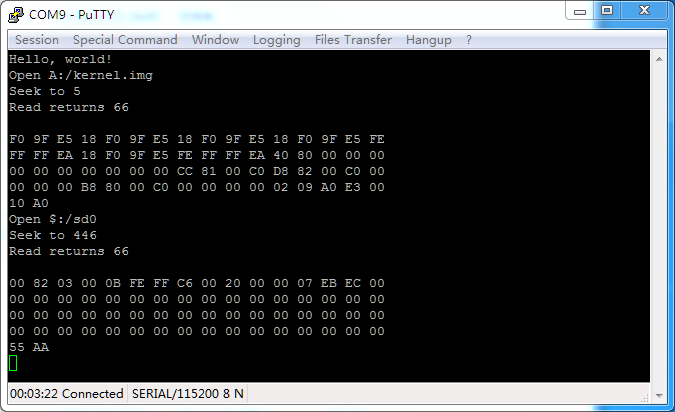
\includegraphics[scale=0.4]{figures/6-1}
\caption{文件系统测试结果}
\label{figure:6-1}
\end{figure}

\clearpage
\ifxetex\else\end{CJK*}\fi
\end{document} 
